\section{Results}
\label{sec:results}

The primary experiment is the Class~A search for a drifting, unresolved
spectral carrier: \NWinA{} fine-channel windows toward \NSysClassA{}
systems. The Class~B search for an unresolved spectral excess is secondary
and carries no drift discrimination: \NWinB{} coarse windows. Together they
are the \NWindows{} windows of the released catalogue. \textbf{No carrier
was found toward any of the \NSystems{} systems searched.} What follows is
first how deep the search reaches, and then what it found and how each
finding was disposed of.

\subsection{Sensitivity: the power at which a carrier would have been
found} \label{sec:pninetysel}

\emph{The sensitivity of this survey is a measured completeness and not a
threshold.} Artificial carriers of known amplitude were added to the real
calibrated ALMA visibilities, each with a random sub-channel phase and a
random drift rate from its window's own grid. They were then recovered
through the unchanged pipeline: extraction, baseline removal, de-drifted
stack, trigger, and the \NCtrl-position spatial screen. The power at which
nine carriers in ten are recovered is $\mathrm{EIRP}_{90}$. It is the only
sensitivity quoted in this paper. It charges for the whole chain the
analysis applies, because a carrier counts as recovered only when it reaches
the trigger \emph{and} the stellar position then outranks every control.

Measured that way, Class~A reaches ninety per cent recovery at
$\mathrm{EIRP}_{90}=\EirpNinetyMultA\,P_{\rm trig}$ and Class~B at
$\EirpNinetyMultB\,P_{\rm trig}$. Here $P_{\rm trig}$ is the window's own
$5\sigma$ trigger power. In absolute terms the median Class~A window reaches
$\EirpNinetyWinMedA$\,W of equivalent isotropic radiated power. The median
system, on its best window, reaches $\EirpNinetySysMedA$\,W, with a spread
across systems of $\EirpNinetySysLoA$--$\EirpNinetySysHiA$\,W
(Fig.~\ref{fig:classasens}a); that per-system median is the figure quoted in
the abstract and in the conclusions. Statistical and systematic terms
combine to one interval, $-\EirpNinetyPctLo$ to $+\EirpNinetyPctHi$ per cent, in which
the largest systematic is the \BudDominant{} term
(Table~\ref{tab:p90budget}). Two one-sided biases cannot be added to an
error and are carried separately; together they are $\EirpNinetyDecorPctLo$ to
$+\EirpNinetyDecorPctHi$ per cent.

\emph{The completeness is measured directly for the injected
configurations and transferred to the rest of the sample, and that transfer
is the dominant caveat on the numbers above.} Carriers were injected
directly into \NInjWinA{} of the \NWinA{} Class~A windows, because every
injected window is re-extracted and re-searched end to end at each
amplitude; the recovered ratio was then transferred to the remaining
\NTransferWinA. The spread of that ratio across the \BudTransN{} windows
that were injected into directly is measured rather than assumed, and it is
carried as the largest single term in the budget rather than removed; it, and
the \BudTransNTransferred{} windows it is transferred to, are the first row
of Table~\ref{tab:p90budget}. Taken with the instrumental terms it puts every
$\mathrm{EIRP}_{90}$ in this paper inside
$\times\EirpNinetyFacLo$--$\times\EirpNinetyFacHi$ of its quoted value, which
is the same interval as the per cent figures above and not a second one. The one
term that is worse for a single star than for the sample is the stellar
position: measured from Gaia parallaxes for \BudPlxNStar{} catalogue stars,
the worst fractional distance error is \BudPlxWorstPct{} per cent, toward
\BudPlxWorstStar. Every value above should therefore
be read as an upper bound on reach rather than a central estimate. Two
further properties of the measurement bound how far it can be pushed. First,
recovery does not reach unity: a bright source at the stellar position leaks
through the dirty beam into the control ring and raises the control maximum
with it, from $\SelCtrlClean\sigma$ on an uninjected pass to
$\SelCtrlTopRung\sigma$ at the brightest rung. Second, the
ninety-per-cent point lies near the end of the injected ladder, so it is the
power at which the measurement runs out rather than a sharp threshold.

\begin{table}
\centering
\scriptsize
\caption{The $\mathrm{EIRP}_{90}$ error budget. The first two rows are
two-sided and combine in quadrature to the one interval quoted in the text,
$-\EirpNinetyPctLo$ to $+\EirpNinetyPctHi$ per cent, of which the larger contribution
is \BudDominant. The decorrelation term is a one-sided bias declared from
the literature rather than measured here, and is therefore quoted apart
from the interval rather than added to it: an uncorrected bias is not an
error bar. Every row is a fractional effect on
$\mathrm{EIRP}_{90}$, so the budget applies unchanged to every limit in
this paper.}
\label{tab:p90budget}
%% The generated fragment's first column plus its p{0.44\columnwidth} origin
%% column overrun the measure by 13.9 pt at \scriptsize.  Narrowed here, by
%% font size and column separation, rather than by hand-editing a fragment
%% whose header says not to; the proper fix is the generator's column spec.
\tiny
\setlength{\tabcolsep}{2pt}
%% GENERATED by numbers_v410.py -- do not hand-edit.
\begin{tabular}{@{}l@{~}>{\raggedright\arraybackslash}p{0.44\columnwidth}@{~}r@{}}
\hline
Term & Origin & $\Delta\mathrm{EIRP}_{90}$ (\%) \\
\hline
Window-to-window transfer & bootstrap over the 21 directly injected windows; this term \emph{is} the campaign statistics & $-22/+8$ \\
Instrumental & flux scale, parallax and visibility scale, in quadrature & $\pm9$ \\
\hline
\emph{Combined} & in quadrature & $-23/+12$ \\
\emph{as a factor on} $\mathrm{EIRP}_{90}$ & & $\times0.77$--$\times1.12$ \\
\hline
\multicolumn{3}{@{}l}{\emph{A one-sided bias, quoted apart from the interval}} \\
Decorrelation & injected tones suffer none; declared, not measured in this work & $-12/+17$ \\
\hline
\end{tabular}

\end{table}

\begin{figure*}
\centering
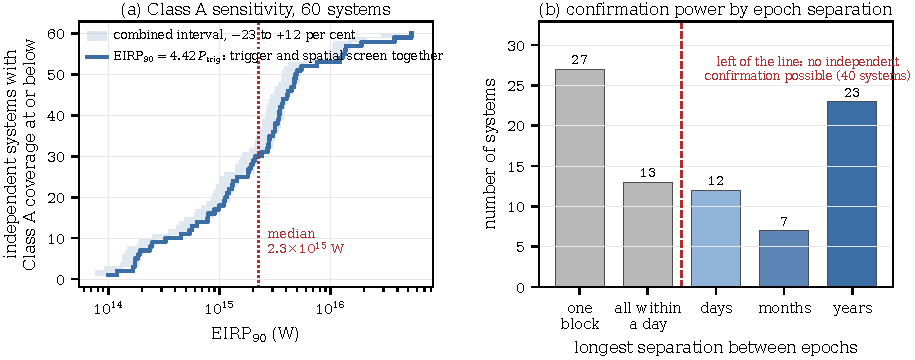
\includegraphics[width=0.92\textwidth]{figures/classa_sensitivity.pdf}
\caption{\emph{(a)}~Class~A sensitivity: the cumulative number of systems
whose best window reaches a given $\mathrm{EIRP}_{90}$, the power at which
nine carriers in ten are recovered through the trigger and the spatial
screen together. The shaded band is the combined interval of
Table~\ref{tab:p90budget}. \emph{(b)}~The temporal selection function:
systems grouped by the longest separation between their searched epochs, an
independent epoch being a separation of more than \EpSep{} day.
\textbf{For the \EpOne{} systems observed in a single block, and the
\EpSameDay{} whose blocks all fall within one day --- left of the dashed
line --- independent confirmation was not possible at all}, whatever the
sensitivity in panel~(a). Recurrence over years can be tested for
\EpYears{} systems of \EpTot.}
\label{fig:classasens}
\end{figure*}

\subsection{The nearest stars: Barnard's Star and Wolf~359}
\label{sec:barnardswolf}

Barnard's Star is the second-nearest stellar system, and Wolf~359 the third
if brown dwarfs are excluded. To our knowledge these are the first
millimetre or submillimetre technosignature limits for either; the searches
checked are \citet{Enriquez2017}, \citet{Price2020} and
\citet{Margot2023}. Both are non-detections. \emph{Both limits come from the
secondary Class~B experiment and not from the carrier search}: the archive
holds only coarse Band~6 windows toward these two stars, so neither is
searched for a drifting carrier and neither constrains one. What is
constrained is an unresolved spectral excess. Quoted on the
$\mathrm{EIRP}_{90}$ convention of \S\ref{sec:pninetysel}, Barnard's Star
reaches $\EirpNinetyBarnLo$--$\EirpNinetyBarnHi$\,W over \NWinBarn{}
windows. Wolf~359 reaches
$\EirpNinetyWolfLo$--$\EirpNinetyWolfHi$\,W over \NWinWolf.

\subsection{Threshold crossings and how each was disposed of}
\label{sec:technosearch}

\emph{The result is a chain of four tests, and it is read in one direction.}
Of the \NWindows{} windows, \NCross{} contain a channel\,$\times$\,drift
cell at the stellar position reaching $T\geq5$. Such a cell is a
\emph{threshold crossing}. The stellar-frame molecular-line mask,
$\pm\MaskHalfKms$\,km\,s$^{-1}$ wide and fixed before any crossing was
classified, identifies \NAttributed{} of them as carbon monoxide.
\NUnattributed{} are unattributed by that test, and every crossing is in one
column or the other. Of the unattributed, \NUnattrRankFlagged{} outrank
all \NCtrl{} control positions in their own window. Neither of those two
recurs in any later epoch covering its frequency. \textbf{No crossing
survives the chain, and this survey reports no detection.}
Figure~\ref{fig:chain} carries the chain with the number surviving each
step, Table~\ref{tab:ledgersum} the same five counts, and
Table~\ref{tab:ledger} the crossing-by-crossing ledger behind them.

\begin{table}
\centering
\footnotesize
\caption{The result in five counts, each read from the rows of
Table~\ref{tab:ledger} so that the two cannot disagree. The line
attribution is evaluated in the stellar frame at the adopted
$\pm\MaskHalfKms$\,km\,s$^{-1}$ half-width, and the last two lines are the
spatial screen and the recurrence test applied in that order.}
\label{tab:ledgersum}
\scriptsize
%% GENERATED by ledger_v410.py -- do not hand-edit.
\begin{tabular}{@{}lr@{}}
\hline
Quantity & Observed \\
\hline
Threshold crossings & 56 \\
Line-attributed ($|\Delta v|\leq50$\,km\,s$^{-1}$, stellar frame) & 18 \\
Unattributed & 38 \\
\quad outranking all spatial controls & 2 \\
\quad recurring at a second epoch & 0 \\
\hline
\end{tabular}

\end{table}

\emph{The mask is informative rather than permissive, and its half-width is
not a tuned parameter.} The width follows from the Keplerian velocity bound
on circumstellar gas in these systems, and doubling it changes none of the
counts above (Appendix~\ref{app:linemask}). Evaluated in the stellar frame
the mask attributes \NAttributed{} crossings, where its occupancy of the
searched band would give \LgExpAttr{} by chance coincidence alone. The
attributions are therefore a kinematic result and not an accident of
bandwidth.

\subsubsection{Most of the crossings are expected by chance}
\label{sec:trigunif}

A $5\sigma$ trigger is a threshold on a statistic and not a false-alarm
rate: the number of searched channel\,$\times$\,drift cells per window spans
several decades, so a common threshold buys very unequal protection.
Summing each window's own measured false-alarm probability over the covered
Class~A windows gives \RsevChanceExp{} expected unattributed Class~A
crossings, against \RsevChanceObsAUnattr{} observed. \emph{About two thirds
of the crossings this survey reports are expected by chance}, which is why
the chain never treats a crossing as a detection and why no artefact
hypothesis is needed to account for their number.

\subsubsection{One execution block accounts for four of the crossings}
\label{sec:bdblock}

\BdNCross{} crossings belong to \BdStar{} (\BdAlias), with the highest
statistics in the survey outside $\beta$~Pictoris and HD~48370. All
\BdNCrossBlock{} lie in one ACA execution block, \texttt{\BdBlock}, in which
the whole field is above threshold: \BdNCtrlAbove{} of \BdNCtrl{} control
positions exceed $T=5$, against a survey median control maximum of
\BdSurvCtrlMed. The single-integration noise is as predicted
(\BdRmsMeas\,Jy against \BdRmsPred\,Jy), but the residual does not integrate
down; a jackknife on the channel mean gives \BdJack\,Jy against
\BdThermal\,Jy thermal. A slow drift common to every channel and every
position therefore inflates the statistic across the field. The
\BdNSibling{} sibling executions of the same field, with the same array and
the same spectral setup, reach a maximum of $T_\star=\BdSibTMax{}$ and
produce no crossing. \emph{The median of the control ensemble, not its
maximum, is the quality criterion this kind of search needs.} We report it
as a diagnostic and do not adopt it as a cut, because a cut strict enough to
remove this block would also remove the HD~48370 carbon-monoxide control.

\subsubsection{Stellar flares are excluded by a broadband prediction}

The hosts are not a quiet sample: \HostNActive{} of \HostNTot{} carry
activity indicators, and magnetically active stars do produce coherent
bursts at centimetre wavelengths. A millimetre flare, however, raises every
channel of a window by the same flux density. A flare able to produce a
$5\sigma$ single-channel crossing must therefore produce a $5\sqrt{N}\sigma$
continuum event in the same integrations. Over the \FlNCont{} crossings with
a recoverable continuum measurement that prediction runs
\FlPredLo--\FlPredHi$\sigma$, while the observed continuum statistic has
median \FlObsMed{} and $|Z|<3$ in \FlNQuiet{} of \FlNCont. One block settles
it directly. \FlEgStar{} \texttt{\FlEgEb} contains both a crossing
($T_\star=\FlEgT$) and the published millimetre flare of
\citet{MacGregor2020}. In the crossing's own time window the continuum is
raised at $Z=\FlEgContZ$, while the crossing's de-drifted track reaches only
$Z_{\max}=\FlEgTrackZ$. \emph{A real, bright, independently published
millimetre flare in the same data contributes \FlEgContrib$\sigma$ to the
single-channel statistic.}

\subsection{$\beta$~Pictoris: an astrophysical positive control, and the
obstacle it identifies} \label{sec:bpicval}

\emph{A search that finds nothing must show that it could have found
something, and the survey's strongest features show exactly that.} The
frozen pipeline recovers the $\beta$~Pictoris circumstellar carbon monoxide
blind, without being told the disc is there. It recovers it in two
rotational transitions and in \NStageOneBpicEb{} independent execution
blocks spanning \BpBaselineYr\,yr: \BpicNFlagThree{} Band~3 windows at
$T_\star$ up to \BpicBThreeTsym, and \BpicNFlagSix{} Band~6 windows at
\BpicBSixTsym. The identification is kinematic and does not rest on those
statistics. Carried through the frame chain, the Band~3 and Band~6 crossings
lie \StelBpicThree{} and \StelBpicSix\,km\,s$^{-1}$ from the stellar
systemic velocity, within \BpicMaxAbsStel\,km\,s$^{-1}$ of it. They lie in
the two lowest CO transitions of a star with mapped circumstellar CO
\citep{Dent2014,Matra2017}. The Band~3 peaks agree across blocks to
\BpRecThreeTuneChanMax{} channel once each block's own tuning is removed, so
any apparent drift is far below the grid searched. The alternative reading
requires a transmitter placed by coincidence at matched offsets from two CO
transitions of one star.

$\beta$~Pictoris is also the control that shows the recurrence test of
\S\ref{sec:etacrv} working in the positive direction. Every
$\beta$~Pictoris carbon-monoxide feature the search flagged is recovered in
an independent execution block, and the screened Band~6 window returns
$T_\star=\BpRecTTwo{}$ in the second block of its own recurrence set. A
non-recurrence elsewhere means nothing unless the same machinery recovers a
repeat where one exists.

\emph{One of those blocks is a counterexample, and it is the more useful
half of the control.} In it the control ring is brighter than the star, and
several of the \NCtrl{} control positions exceed the stellar statistic, so
the spatial screen rejects a window containing carbon monoxide that is known
to be real and known to be centred on the star. The disc is resolved on the
scale of the primary beam in that configuration, which is exactly the
geometry the screen is built to reject. \textbf{The screen is therefore not
a test of authenticity but a test of compactness}, and on a real,
spatially extended source it fails in the conservative direction. That is a
stronger statement than a clean positive control would be, because it bounds
the screen's reach as well as demonstrating it (Fig.~\ref{fig:bpiccontrol}).

\begin{figure}
\centering
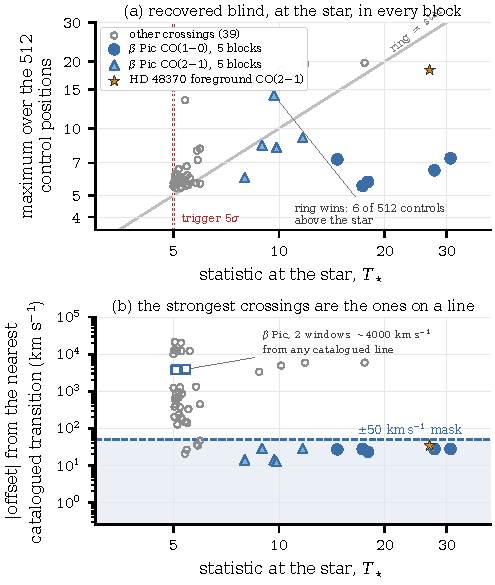
\includegraphics[width=0.88\columnwidth]{figures/bpic_control.pdf}
\caption{The $\beta$~Pictoris positive control, in both directions.
\emph{(a)}~The spatial screen. One point per execution block in which the
blind search recovers circumstellar carbon monoxide, plotted as the stellar
statistic against the maximum over that window's \NCtrl{} control positions:
the \NStageOneBpicEb{} blocks in which the star outranks every control, and
one further block in which the ring wins. \emph{The control is that the
search recovers a real narrow line at a stellar position, in two transitions
and in every one of these blocks.} It is not that the star outranks the ring
everywhere. In block \texttt{\BpCtrlBlock}, Band~\BpCtrlBand, the control
ring reaches \BpCtrlRingMax{} against \BpCtrlStar{} at the star, with
\BpCtrlNAbove{} of the \BpCtrlNCtrl{} control positions above it, so the
screen rejects a window holding carbon monoxide that is real, centred on the
star and independently mapped. The disc is resolved on the scale of the
primary beam in that configuration, which is the geometry the screen is
built to reject, so \textbf{the screen measures compactness and not
authenticity} (\S\ref{sec:bpicval}). \emph{(b)}~Line confusion, which is
what makes the screen's job hard. The \BpicPanelNCo{} $\beta$~Pictoris
carbon-monoxide crossings are plotted by their velocity offset from the
nearest catalogued transition, against the mask half-width, with the
adopted $\pm\MaskHalfKms$\,km\,s$^{-1}$ marked. All of them land
\BpicDvCoLo--\BpicDvCoHi\,km\,s$^{-1}$ from CO, well inside the mask, while
the two CS($5{\to}4$) crossings of the same star sit
\BpicDvCsLo--\BpicDvCsHi\,km\,s$^{-1}$ from anything catalogued and are not
attributed at any width. The survey's \BpicPanelNOther{} other crossings are
in grey, with HD~48370 marked. \emph{A crossing is identified by where it falls in this plane and
not by how strong it is}, which is why the line mask and not the trigger is
the productive test.}
\label{fig:bpiccontrol}
\end{figure}

HD~48370 is the complementary case and is equally instructive. Its crossing
reaches $T_\star=\HdTsym$, but the control ring rises with the star, to
\HdRingMax, as emission filling the primary beam does. The velocity matches
the prominent CO($2{\to}1$) that \citet{Cataldi2023} report toward the
source and flag as possible foreground cloud emission. The block's
$^{13}$CO($2{\to}1$) window is bright at the ring and faint at the star.
Extended line emission is therefore rejected by the same spatial statistic
that promotes $\beta$~Pictoris.

\emph{Taken together, these two results identify the dominant obstacle for
millimetre technosignature searches, and it is not sensitivity.} The
strongest apparent signals in this survey are circumstellar and foreground
molecular emission, and \NAttributed{} of the \NCross{} crossings are
molecular lines. The mask that removes them costs almost nothing in
bandwidth: \MaskUnionPct{} per cent of the unique-frequency union and
\MaskGrossPct{} per cent of gross bandwidth, over \MaskNSpecNew{} species.
It is nevertheless the single most productive test in the chain. The warning
for future work is about line lists rather than about depth. Against a wide
spectral-line harvest, rather than the \MaskNSpecNew-species mask used here,
a \emph{uniformly random} frequency in one of these windows falls within
$\pm\MaskHalfKms$\,km\,s$^{-1}$ of some catalogued transition most of the
time. A near coincidence is therefore the default outcome and carries no
information either way. Any survey at these frequencies that quotes a line
coincidence should quote the occupancy of the list it used.

\subsection{The two crossings that pass the spatial screen}
\label{sec:chaingap}

\NUnattrRankFlagged{} of the \NCross{} crossings are both unattributed and
outrank every control in their own window, and both are in Band~7.
\EpGapStar, in block \EpGapEb, reaches $T_\star=\EpGapT$; \EpOutStar, in
block \EpOutEb, reaches $T_\star=\EpOutT$. Their frequencies and velocity
offsets are in Table~\ref{tab:ledger}. Neither lies within
$\pm\MaskHalfKms$\,km\,s$^{-1}$ of a masked transition in its star's own
frame. \emph{Each is disposed of by the same thing: its own later epochs.}
\EpGapStar{} has \EpGapNRep{} further execution blocks covering the event's
frequency, and the largest statistic anywhere in them is
$T_\star=\EpGapRepTMax$. \EpOutStar{} has \EpOutNRep{} such blocks. The
deepest was taken two hours later and is \CpRecDeeperPct{} per cent deeper
in noise; a carrier persisting at the discovery flux would have given
$T_\star=\CpRecExpT$ there, and the measured value is \CpRecT. That excludes
persistence at \CpRecExclCond$\sigma$. Two further measurements close
\EpOutStar{} independently of any line list. The feature is wider at the
recovered drift than the instrumental response, whereas a warm circumstellar
sulphur line would be resolved. And CO($3{\to}2$) lies in the same window
and is absent, below a limit fainter than the crossing itself.

\subsubsection{The visibility fit, and why it is not the discriminant}
\label{sec:vistest}

\LgNFit{} of the \NCross{} crossings were also re-measured in the visibility
domain, by phase rotating to the star and following the recovered drift; for
the remainder the fit is outstanding rather than negative. That result is
reported in the data release beside the chain rather than inside it, because
it is a consistency check on position and epoch. The reason is structural: a
noise maximum \emph{at} the stellar position has flux at the stellar
position. At the trigger it therefore returns a real part close to the
trigger itself, and carries almost nothing beyond the trigger that selected
it. The injection campaign measures this directly. For real sources at the
star the two estimators track to within about ten per cent, and in the bin
the unattributed crossings occupy injected sources return
${\rm Re}/\sigma=\RsevReAtFiveMeanA\pm\RsevReAtFiveSdA$. The values returned
by the two screened crossings are consistent with a real source and do not
exclude one. \textbf{The discriminating evidence is the line mask, the
spatial screen and recurrence, and not the visibility fit.}

\subsection{Recurrence is the confirmation criterion, and the sample barely
supports it} \label{sec:etacrv}

\emph{A persistent transmitter should be there the next time the same
frequency is observed.} That is the confirmation criterion used here, and it
is applied in the star's own frame. The expected channel is computed by
correcting the observed frequency for the Earth's motion at the repeat epoch
and for the star's systemic velocity. The statistic is then read at that
channel, at a single drift rate. Recurrence has been evaluated for
\LgNRecurTested{} crossings over \LgNRecurRepeats{} covering repeat blocks.
The largest statistic returned anywhere in them is
$T_\star=\LgRecurTMax$, against a trigger of 5. \emph{Nothing recurs.}

Those repeat epochs include an archival extension searched with the same
frozen pipeline, after the detection statistic and the line mask were fixed:
\ExtBlocks{} further execution blocks, \ExtWindows{} windows toward
\ExtStars{} stars in \ExtSystems{} systems. Every block in it is repeat
coverage of a star and a tuning already in the sample, so it adds no star,
no system and no frequency. What it adds is epochs. It is reported
separately from the primary census, because every statistic above rests on a
denominator and a crossing list fixed before these data were examined.
Merging the two would destroy that property. Nor is the archive exhausted:
\FateNoCal{} further in-scope blocks expose no pipeline calibration product
in the ALMA delivery at all, so the recurrence statements rest on the epochs
actually in hand (\S\ref{sec:coverage}).

$\eta$~Crv shows why the frame correction is not a detail. Its crossing at
\VnEcrFreq\,GHz is covered by exactly \VnEcrNCover{} epochs in the whole
archive, and the second is \VnEcrDepthRatio{} times deeper than the
discovery. Matching in the stellar frame moves the expected cell by
\VnEcrDchan{} channels, so a sky-frequency test would have examined the
wrong channel. At the matched cell the statistic is \VnEcrOtherT, where a
carrier persisting at the discovery flux would have given \VnEcrTPers.
\emph{A persistent source is excluded at \VnEcrExcl$\sigma$ from one epoch},
which carries \VnEcrNeff{} equivalent discovery epochs of sensitivity.

\emph{The limitation belongs in the same breath as the criterion.} Only part
of the sample has repeat epochs separated well enough to test persistence at
all. \EpOne{} of the \EpTot{} systems were observed in a single execution
block, and \EpSameDay{} have all their blocks within one day. For none of
those systems was confirmation possible, whatever the sensitivity
(Fig.~\ref{fig:classasens}b). Only \EpYears{} systems can be tested over
years, and for the two screened crossings the usable baselines are
\UnattSepMinD--\UnattSepMaxD\,d. \textbf{These tests exclude a carrier
persistent over hours to days; they bound no duty cycle measured in months
or years.} The constraint on an intermittent transmitter is accordingly much
weaker than the constraint on a continuous one. Repeat coverage is also
matched on the window rather than on the crossing frequency, which the
release records only where the pipeline stored a peak.

\begin{table*}
\centering
\caption{\textbf{The crossing ledger.} Every one of the \NCross{} threshold
crossings: the star, its execution block, the ALMA band, the crossing
frequency, the search statistic $T_\star$, the molecular transition the
stellar-frame $\pm\MaskHalfKms$\,km\,s$^{-1}$ mask attributes it to, the
velocity offset $\Delta v$ from that transition, and its disposition.
Frequencies marked $^{*}$ are window centres, the crossing frequency not
having been recorded. Block identifiers omit the constant \texttt{A002\_}
prefix. Dispositions are \textbf{A} attributed to a molecular transition,
\textbf{U1} unattributed and outranked by at least one control position, and
\textbf{U2} unattributed, outranking every control, tested for recurrence
and absent in the repeat epochs.}
\label{tab:ledger}
\tiny
%% GENERATED by ledger_v410.py -- do not hand-edit.
%% One row per threshold crossing, one epoch convention, stellar-frame attribution.
\begin{tabular}{@{}l@{~}l@{~}c@{~}r@{~}r@{~}c@{~}l@{~}r@{~}l@{}}
\hline
Star & block & B & $\nu$ (GHz) & $T_\star$ & scr & line & $\Delta v$ & disposition \\
\hline
$\beta$~Pic & Xf5d76d\_Xeb8 & 3 & 114.8292 & 30.765 & Y & CO(1-0) & -2.9 & attributed \\
$\beta$~Pic & Xf5d76d\_Xe19 & 3 & 114.8292 & 27.684 & Y & CO(1-0) & -2.9 & attributed \\
HD 48370 & Xc26103\_X155a & 6 & 230.5117 & 26.834 & Y & CO(2-1) & -17.8 & attributed \\
$\beta$~Pic & Xf4df6f\_Xc7 & 3 & 114.8309 & 17.907 & Y & CO(1-0) & -2.9 & attributed \\
BD+05 1668 & Xc7fa6f\_X28a8 & 6 & 240.1016 & 17.519 & n & CS(5-4) & -5912.4 & unattributed; below rank screen \\
$\beta$~Pic & Xf5d76d\_Xcc5 & 3 & 114.8292 & 17.288 & Y & CO(1-0) & -2.9 & attributed \\
$\beta$~Pic & Xf5d76d\_X32f1 & 3 & 115.2606 & 14.654 & Y & CO(1-0) & -2.3 & attributed \\
BD+05 1668 & Xc7fa6f\_X28a8 & 6 & 224.7422 & 11.868 & n & 13CO(2-1) & +5912.5 & unattributed; below rank screen \\
$\beta$~Pic & Xd9668b\_X3a90 & 6 & 230.5161 & 11.681 & Y & CO(2-1) & -3.4 & attributed \\
BD+05 1668 & Xc7fa6f\_X28a8 & 6 & 226.7422 & 10.136 & n & CO(2-1) & -4931.3 & unattributed; below rank screen \\
$\beta$~Pic & X6f1341\_X1484 & 6 & 230.5284 & 9.832 & Y & CO(2-1) & -3.3 & attributed \\
$\beta$~Pic & X7116f1\_X1785 & 6 & 230.5272 & 9.677 & n & CO(2-1) & -2.6 & attributed \\
$\beta$~Pic & Xd9668b\_Xa9df & 6 & 230.5160 & 8.948 & Y & CO(2-1) & -3.5 & attributed \\
BD+05 1668 & Xc7fa6f\_X28a8 & 6 & 242.1953 & 8.784 & n & CS(5-4) & -3349.7 & unattributed; below rank screen \\
$\beta$~Pic & Xa7a216\_X23e4 & 6 & 230.1117 & 7.988 & Y & CO(2-1) & -3.6 & attributed \\
61 Vir & Xc079b5\_X82f & 7 & 346.3138 & 5.958 & Y & CO(3-2) & +457.1 & unattributed; rank-flagged \\
HD 285968 & Xd98580\_X3bf6 & 6 & 230.5021 & 5.956 & n & CO(2-1) & +8.7 & attributed \\
HD 285968 & Xdb7ab7\_X5b4e & 6 & 230.5116 & 5.868 & n & CO(2-1) & +8.7 & attributed \\
HD 285968 & Xdb4b9a\_X108f & 6 & 230.5100 & 5.835 & n & CO(2-1) & +8.7 & attributed \\
CP$-$72 2713 & Xff0235\_X4a6d & 7 & 344.2697 & 5.809 & Y & CO(3-2) & -1299.9 & unattributed; rank-flagged \\
HD~139084~B & Xcd8029\_Xb6b0 & 7 & 345.8241 & 5.763 & n & CO(3-2) & +24.3 & attributed \\
HD 14055 & Xfff3d8\_Xd46 & 7 & 331.7699 & 5.575 & n & CO(3-2) & -12163.2 & unattributed; below rank screen \\
HD 23484 & X10b22d7\_X2445 & 6 & 230.7904 & 5.520 & n & CO(2-1) & +341.5 & unattributed; below rank screen \\
HD 161868 & Xff45a6\_X10ca8 & 7 & 345.6338 & 5.481 & n & CO(3-2) & -127.4 & unattributed; below rank screen \\
HIP 10679 & Xa95c04\_X14cd & 6 & 220.4185 & 5.456 & n & 13CO(2-1) & +6.1 & attributed \\
HD~14055 & X11adad7\_X25c5e & 7 & 345.4564 & 5.448 & n & CO(3-2) & -317.1 & unattributed; below rank screen \\
HD 207129 & Xc19d6f\_X5706 & 6 & 230.4226 & 5.433 & n & CO(2-1) & -170.3 & unattributed; below rank screen \\
$\beta$~Pic & Xd9668b\_X3a90 & 6 & 241.7512 & 5.420 & n & CS(5-4) & -3873.0 & unattributed; below rank screen \\
HR~1010 & Xc6fa08\_X1053 & 6 & 230.5133 & 5.410 & n & CO(2-1) & -32.0 & attributed \\
ALMA J153702653-33192492 & Xff0235\_X8392 & 6 & 230.5222 & 5.405 & n & CO(2-1) & +1.6 & attributed \\
HD 110411 & Xe45e29\_Xb7d4 & 6 & 219.4538 & 5.393 & n & C18O(2-1) & -169.8 & unattributed; below rank screen \\
HD 31392 & X129754b\_X6946 & 6 & 231.1998 & 5.289 & n & CO(2-1) & +890.8 & unattributed; below rank screen \\
HD 14055 & Xff99e1\_X24be0 & 7 & 331.7078 & 5.277 & n & CO(3-2) & -12217.9 & unattributed; below rank screen \\
AU Mic & Xa42f75\_X319 & 6 & 230.6864 & 5.274 & n & CO(2-1) & +172.3 & unattributed; below rank screen \\
HD 69830 & X12209f7\_X16edb & 7 & 322.4325 & 5.259 & n & CO(3-2) & -20244.2 & unattributed; below rank screen \\
ALMA J153702653-33192492 & Xfe62c1\_X398 & 6 & 216.1844 & 5.228 & n & SiO(5-4) & -1244.6 & unattributed; below rank screen \\
AU Mic & X899169\_X1838 & 6 & 230.8252 & 5.221 & n & CO(2-1) & +379.0 & unattributed; below rank screen \\
HD 14055 & Xff99e1\_X2c3bb & 7 & 345.5256 & 5.186 & n & CO(3-2) & -237.9 & unattributed; below rank screen \\
HD 14055 & Xfffde1\_X3835 & 7 & 345.0099 & 5.177 & n & CO(3-2) & -684.0 & unattributed; below rank screen \\
HD 14055 & Xff99e1\_X2b2ee & 7 & 344.7007 & 5.175 & n & CO(3-2) & -953.3 & unattributed; below rank screen \\
LHS 1140 & Xd9d7c7\_X6fd2 & 6 & 230.6355 & 5.136 & n & CO(2-1) & +115.5 & unattributed; below rank screen \\
HD 10647 & Xff294f\_Xaf70 & 7 & 331.6570 & 5.120 & n & CO(3-2) & -12224.3 & unattributed; below rank screen \\
CD$-$57 1054 & Xcf525f\_X5aa4 & 7 & 346.5099 & 5.108 & n & CO(3-2) & +633.3 & unattributed; below rank screen \\
ALMA J153702653-33192492 & Xf8f6a9\_X10359 & 6 & 217.7292 & 5.091 & n & H2CO & -680.2 & unattributed; below rank screen \\
GJ 849 & Xd9668b\_X841a & 6 & 230.8769 & 5.090 & n & CO(2-1) & +416.3 & unattributed; below rank screen \\
ALMA J153702653-33192492 & Xfe62c1\_X398 & 6 & 218.8729 & 5.090 & n & H2CO & +920.7 & unattributed; below rank screen \\
HD 14055 & X1001fdc\_X29ae & 7 & 331.1559 & 5.082 & n & CO(3-2) & -12693.6 & unattributed; below rank screen \\
$\beta$~Pic & Xd9668b\_Xa9df & 6 & 241.8367 & 5.079 & n & CS(5-4) & -3768.4 & unattributed; below rank screen \\
ALMA J153702653-33192492 & Xf8f6a9\_X10359 & 6 & 218.6711 & 5.048 & n & H2CO & +613.8 & unattributed; below rank screen \\
HD 69830 & X12277ed\_X178c6 & 7 & 321.2005 & 5.046 & n & CO(3-2) & -21309.9 & unattributed; below rank screen \\
HR 1010 & Xc66ce1\_Xaa9 & 6 & 230.8348 & 5.044 & n & CO(2-1) & +404.5 & unattributed; below rank screen \\
61 Vir & Xc067f7\_X822 & 7 & 345.5599 & 5.038 & n & CO(3-2) & -197.8 & unattributed; below rank screen \\
HD 170773 & Xff0235\_X8c42 & 7 & 331.0101 & 5.029 & n & CO(3-2) & -12806.8 & unattributed; below rank screen \\
ALMA J153702653-33192492 & Xd9d7c7\_Xbb64 & 7 & 347.2179 & 5.009 & n & CO(3-2) & +1207.8 & unattributed; below rank screen \\
HD~14055 & X1190de8\_Xd526 & 7 & 344.4676 & 5.006 & n & CO(3-2) & -1165.6 & unattributed; below rank screen \\
$\eta$~Crv & X122b6ff\_X1041e & 7 & 357.2815 & 5.006 & n & CO(3-2) & +9929.0 & unattributed; below rank screen \\
\hline
\end{tabular}

\end{table*}


\begin{figure}
\centering
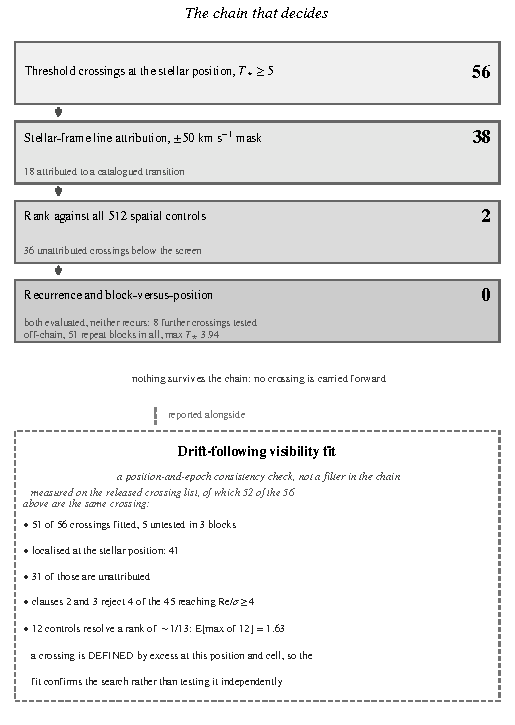
\includegraphics[width=\columnwidth]{figures/chain_v403.pdf}
\caption{The chain that disposes of a threshold crossing, with the number
surviving each step: \NCross{} crossings, \NAttributed{} identified as
carbon monoxide by the stellar-frame line mask, \NUnattributed{}
unattributed, \NUnattrRankFlagged{} outranking every one of the \NCtrl{}
control positions, and none recurring in a later epoch. Every count is read
from the ledger, so the figure and Table~\ref{tab:ledger} cannot disagree.
The visibility fit sits outside the column, because it is evaluated at the
position and in the cell where the search already found an excess
(\S\ref{sec:vistest}).}
\label{fig:chain}
\end{figure}

%% ---------------------------------------------------------------------
%% REQUEST (results owner -> numbers owner).  Eight macros this file uses
%% that the frozen layer does not yet define, all on the adopted
%% trigger-plus-spatial-screen criterion (EirpNinetyMultA = 5.70):
%%   \EirpNinetyWinMedA                      median Class A window, W
%%   \EirpNinetySysLoA \EirpNinetySysMedA \EirpNinetySysHiA
%%                                           per system, best window, W
%%   \EirpNinetyBarnLo \EirpNinetyBarnHi     Barnard's Star, W
%%   \EirpNinetyWolfLo \EirpNinetyWolfHi     Wolf 359, W
%% The \Promote* family (\PromoteMedA, \PromoteSysMedA, ...) is the same
%% quantity on the superseded localisation criterion and is cited nowhere
%% in this file; it is still cited in 03_sample.tex and 07_conclusions.tex,
%% which must move to the names above or the paper will carry two
%% sensitivities again.  \EirpBarnLo/\EirpBarnHi/\EirpWolfLo/\EirpWolfHi
%% are nominal triggers and are no longer quoted here.
%%
%% REQUEST (results owner -> numbers owner).  tab_ledger_v403 must drop
%% nine columns: both visibility-fit epoch groups (Re/sigma, Im/sigma,
%% ctrl, twice), the epoch displacement D, the off-channel column "off",
%% and the "scr" rank flag, whose result is carried by the disposition
%% code.  Eight columns remain: star, block, band, nu, T_star, line, dv,
%% disposition.  \LedgerLegend is replaced by the caption above, so the
%% legend macro is no longer referenced.
%%
%% REQUEST (results owner -> numbers owner).  tab_maskladder.tex now has a
%% home as Table tab:maskladder in this file.  Its fourth column header
%% reads "rank-flagged", a phrase this manuscript has used in both senses;
%% please rename it to "outrank all controls" so the header cannot be read
%% as its own opposite.  The caption states the meaning meanwhile.
%%
%% REQUEST (results owner -> figures owner).  fig:chain MUST BE RE-EMITTED
%% AT SINGLE-COLUMN GEOMETRY.  It is now a \begin{figure} at \columnwidth,
%% not a figure* at 0.98\textwidth, because the section measures 6.0 pp as
%% three full-width floats and 5.0 pp with this one in a column -- the
%% overage was float packing, not words.  chain_v403.pdf is still drawn for
%% full width, so its labels are currently at about half their intended
%% size: PLEASE RE-EMIT FOR ONE COLUMN.  A six-step vertical chain reads
%% better in a column than across a page, so this is the right geometry
%% for it, but the caption, the placement and the artwork must agree and
%% today only two of the three do.  If re-emission is refused, revert this
%% float to figure*/0.98\textwidth and the section is 6.0 pp.
%%
%% REQUEST (results owner -> figures owner).  fig:bpiccontrol.
%%  - GEOMETRY CONFIRMED SINGLE COLUMN.  bpic_control.pdf is 237.6 x 280.7 pt,
%%    i.e. one column wide with the two panels stacked vertically, and the
%%    float is \columnwidth in a \begin{figure}.  Caption and placement
%%    agree; no re-emission at full width is wanted.  Panel (b) gets the
%%    full column width this way, which is what it needs.
%%  - COUNTS I WOULD NOT INVENT.  \NStageOneBpicEb (9) counts the blocks in
%%    which the star outranks every control, so it cannot also count the
%%    points drawn: the ring-wins block is by definition not one of the 9.
%%    The caption therefore says "the 9 ... and one further block" rather
%%    than giving a total.  Four macros would let it say what is drawn:
%%      \BpicPanelNCo     beta Pic CO points in panel (b)        (10)
%%      \BpicPanelNOther  other crossings drawn in grey          (39)
%%      \BpicDvCoLo \BpicDvCoHi   |dv| range of the CO crossings (12-29)
%%      \BpicDvCsLo \BpicDvCsHi   |dv| of the two CS(5-4) crossings
%%    \BpicDvLo/\BpicDvHi existed earlier today and have since been retired.
%%  - COUNTEREXAMPLE NUMBERS, requested and still absent: the ring maximum
%%    (14.13), the stellar statistic (9.68) and the number of the \NCtrl
%%    controls above the star (6) in the ring-wins block.  When they exist
%%    the caption should name that block instead of gesturing at it.
%%
%% REQUEST (results owner -> integrator).  Labels and floats deleted from
%% this file, with the files that still reference them:
%%   sec:linecost     -> sec:bpicval   (06_discussion, app_F, app_I, app_K)
%%   sec:repairedstat -> app:v409      (08_backmatter, app_A, app_M)
%%   eq:tunif         no longer defined anywhere (app_L cites it)
%%   tab:crossdelta   float deleted with the revision-history material;
%%                    app_M_repaired.tex still cites it
%%   tab:clustv409    float deleted; nothing else cites it
%%   fig:ledgervis    no longer cited (float lives in app_K)
%%   tab:hosts        no longer cited from here
%%   app:etacrvrecur  no longer cited from here (app_M still cites it)
%% ---------------------------------------------------------------------
